%%「論文」，「レター」，「レター（C分冊）」，「技術研究報告」などのテンプレート
%% v3.3N [2023/03/30]
%% 1. 「論文」
\documentclass[technicalreport]{ieicej}
%\documentclass[invited]{ieicej}% 招待論文
%\documentclass[survey]{ieicej}% サーベイ論文
%\documentclass[comment]{ieicej}% 解説論文
%\usepackage[dvips]{graphicx}
\usepackage[dvipdfmx]{graphicx,xcolor}
\usepackage[fleqn]{amsmath}
%\usepackage{newtxtext}% 英数字フォントの設定を変更しないでください
%\usepackage[varg]{newtxmath}% % 英数字フォントの設定を変更しないでください
%\usepackage{mathptmx} %Fallback font package
\usepackage{latexsym}
\usepackage{url}
%\usepackage{amssymb}

\setcounter{page}{1}

\field{D} % 情報・システム
\jtitle{鳥獣害対策のための複数台カメラを用いた低コスト通信型警戒システムの開発}
\etitle{Development of a Low-Cost Communication-Based Monitoring System Using Multiple Cameras for Wildlife Damage Control}
\authorlist{%
 \authorentry{佐藤 光汰}{Kota Sato}{aff1}\MembershipNumber{}
 \authorentry{伊東 峻吾}{Shungo Ito}{aff1}\MembershipNumber{}
 \authorentry{単 麟}{Lin Shan}{aff1}\MembershipNumber{}
 \authorentry{松尾 大輔}{Daisuke Matsuo}{aff1}\MembershipNumber{}
 \authorentry{佐藤 真平}{Shimpei Sato}{aff1}\MembershipNumber{}
}
\affiliate[aff1]{信州大学工学部\\ 〒380-8553 長野県長野市若里4-17-1\\ E-mail: 25w6039c@shinshu-u.ac.jp}{Faculty of Engineering, Shinshu University\\ 4-17-1 Wakasato, Nagano, 380-8553 Japan}
%\paffiliate[]{}
%\paffiliate[現在の所属ラベル]{和文所属}
\jalcdoi{???????????}% ← このままにしておいてください

\begin{document}
\begin{abstract}
    %和文あらまし 500字以内
    近年，野生鳥獣による農作物被害が深刻化しており，動物の出現を検知し，撮影画像を即時に通知するトレイルカメラシステムの開発が進められている．
    しかし，従来のシステムは初期導入費や通信費（ランニングコスト）が高価であるという課題に加え，風による草木の揺れ等に起因する誤検知（空撮影）が多く，撮影画像から対象動物を目視で選別する人的労力が大きな障壁となっている．
    本論文では，これらの課題を解決するため，階層的な処理構造を持つ低コスト通信型警戒システムを提案する．
    本システムは，安価な複数のエッジカメラ（ESP32），エッジサーバ（Raspberry Pi），およびクラウドサーバの3層から構成される．
    エッジサーバにおいて撮影画像を集約し，YOLOv8を用いた物体検出により動物が写っている画像のみを選別してクラウドへ送信することで，必要な回線契約数と通信量の削減と人的労力の削減を実現する．
    実証実験の結果，本システムは誤検知等による不要な画像の送信を約80\%削減し，従来システムと比較して通信コストおよび運用労力を大幅に抑制可能であることを示した．
\end{abstract}
\begin{keyword}
    鳥獣被害対策, トレイルカメラ, YOLOv8, ESP32, Raspberry Pi
\end{keyword}
\begin{eabstract}
    In recent years, agricultural damage caused by wildlife has become a serious issue, leading to the development of trail camera systems that detect animal presence and immediately notify users.
    However, conventional systems face challenges such as high initial and running costs, as well as frequent false positives (empty shots) caused by environmental factors like wind-blown vegetation.
    These false positives create a significant barrier due to the manual labor required to sort images visually.
    To address these issues, this paper proposes a low-cost, communication-based monitoring system with a hierarchical processing structure.
    The system consists of three layers: multiple low-cost edge cameras (ESP32), an edge server (Raspberry Pi), and a cloud server.
    The edge server aggregates images from cameras and filters them using YOLOv8-based object detection, transmitting only images containing animals to the cloud.
    This approach reduces the number of required cellular contracts, data traffic, and manual labor.
    Field experiments demonstrated that the proposed system reduces unnecessary image transmission by approximately 80\%, verifying its ability to significantly lower communication costs and operational workload compared to conventional systems.
\end{eabstract}
\begin{ekeyword}
    Wildlife Damage Control, Trail Camera, YOLOv8, ESP32, Raspberry Pi
\end{ekeyword}
\maketitle

\section{まえがき}
近年，ニホンジカやイノシシなどの野生鳥獣による農作物被害は深刻な社会問題となっている．
農林水産省の統計によると，令和6年度の野生鳥獣による農作物被害金額は180億円を超え，鳥獣害対策が急務となっている\cite{maff}．

例えば，動物の出没に合わせて追い払い機器を作動させる，あるいは罠の設置場所を最適化するといった効果的な鳥獣害対策を講じるためには，対象動物が「いつ」「どこに」現れたかという情報を，リアルタイムに把握することが極めて重要である．事後的なデータ回収では対応できない，即時性のある対策が可能となるからである．

これまでの研究や現場でのモニタリングにおいては，PIR（Passive Infrared Ray）センサを搭載した自動撮影カメラ（トレイルカメラ）が広く利用されてきた．
従来のトレイルカメラは通信機能を持たず, 撮影画像をSDカードに記録し，後に回収して確認するのが一般的であったが，近年ではTabakら\cite{Tabak2019}のように深層学習を用いて自動で動物種を識別する試みや，LTEや衛星通信機能を用いて撮影画像を即時にユーザへ通知するシステム\cite{Whytock2023,Patkar2025}も実用化されている．

しかし，既存の通信型トレイルカメラを広範囲な農地や山林に多数展開するには，コストと運用効率の面で課題が残る．
第一に，空撮影による弊害である．
PIRセンサは熱源の移動を検知するため，風による草木の揺れ等にも反応し，動物が写っていない空画像を大量に撮影してしまう．
これにより，ユーザは膨大な撮影画像の中から対象動物が写っている画像を目視で選別する必要があり，多大な労力を要する．
第二に，導入・運用コストの問題である．
リアルタイムな通知を行うためにLTE通信機能付きカメラを利用する場合，カメラ自体の価格が高価であることに加え，カメラ1台ごとに回線契約が必要となる．
そのため，広域で監視網を構築すると，初期コストとランニングコストが高価となり，一般の農家や自治体にとって導入の障壁となっている．

本研究では，安価な複数のエッジカメラ，エッジサーバ，およびクラウドサーバからなるトレイルカメラシステムを提案する．
本システムは，エッジサーバにおいて複数のカメラからの画像を集約し，単一の回線契約での運用を可能とすることで，通信コストを大幅に削減する．
また，エッジサーバ上で軽量なAIモデルを用いた画像認識を行うことで，動物が写っている画像のみを送信し，通信量の抑制とユーザによる確認作業の負担軽減を実現する．
加えて，システム構成要素に汎用的な安価なデバイスを選定しつつ，広域をカバーする費用対効果の高い監視網の構築を可能とする．

本論文の構成は以下の通りである．
第2章では関連研究について述べ，第3章では提案システムの詳細について説明する．
第4章では提案システムの実験評価を行い，第5章で実験結果に対する考察を述べる．最後に第6章で本論文を締めくくる．

\section{関連研究}
野生動物モニタリングの効率化において，深層学習の適用は近年注目されているアプローチである．
Tabakら\cite{Tabak2019}は，大規模なカメラトラップ画像データセットを用いてCNN（Convolutional Neural Networks）モデルを学習させ，98\%以上の精度で動物種の自動識別が可能であることを示した．
また，Fennellら\cite{Fennell2022}は，物体検出モデルを用いることで動物と人間を正確に区別し，プライバシー保護と調査効率の向上を両立させている．
しかし，これらの研究の多くは，SDカード回収後の事後処理や，撮影された全画像をクラウドへ送信して処理することを前提としており，通信帯域が限られ，かつ即時性が求められる鳥獣害対策の現場においては適用が困難である．

リアルタイム性を重視した研究として，Whytockら\cite{Whytock2023}は衛星通信を利用した即時アラートシステムを開発したが，通信コストが極めて高く，一般の農家や自治体が広範囲に導入するには障壁が高い．
一方，エッジデバイス上で推論を行う試みとして，Patkarら\cite{Patkar2025}やRahmanら\cite{Computers2025}はRaspberry Pi等のシングルボードコンピュータを用いた高性能な監視システムを提案している．
しかし，これらのデバイスは消費電力が比較的大きく，商用電源が得られない山間部等での長期運用には，大型のバッテリーやソーラーパネルが必要となり，機材コストと設置の難易度を増大させる．

省電力化のアプローチとして，Saitoら\cite{IEICE2020}はESP32等の安価なマイコン上での軽量CNNモデルの動作検証を行い，低消費電力なノード構築の可能性を示した．
しかし，彼らの研究は単体ノードでの検証に留まり，複数ノードの連携や，実際のフィールド環境における通信網の構築，および誤検知画像の実践的なフィルタリング効果については十分に検証されていない．

本研究の独自性は，撮影に特化した安価な「エッジカメラ」と，画像集約・画像選別を担う「エッジサーバ」、高度な画像解析・ユーザ通知を担う「クラウドサーバ」の3層構造にした点にある．
これにより，カメラごとの回線契約を不要とし，広域展開における「導入・運用コストの削減」と，誤検知排除による「運用効率の向上」を両立させる．

\section{提案システム}
本章では，提案システムのアーキテクチャおよび詳細な処理フローについて述べる．

\subsection{システム構成}
提案システムの全体構成を図\ref{fig:system}に，データ処理フローを図\ref{fig:flow}に示す．
本システムは，以下の3層構造から成る．

\begin{enumerate}
    \item \textbf{エッジカメラ}: 画像取得・エッジサーバへの転送
    \item \textbf{エッジサーバ}: 画像集約・軽量AI画像選別・クラウドサーバへの転送
    \item \textbf{クラウドサーバ}: 高度なAI画像解析・データ蓄積・ユーザ通知
\end{enumerate}

\begin{figure}[tb]
    \centering
    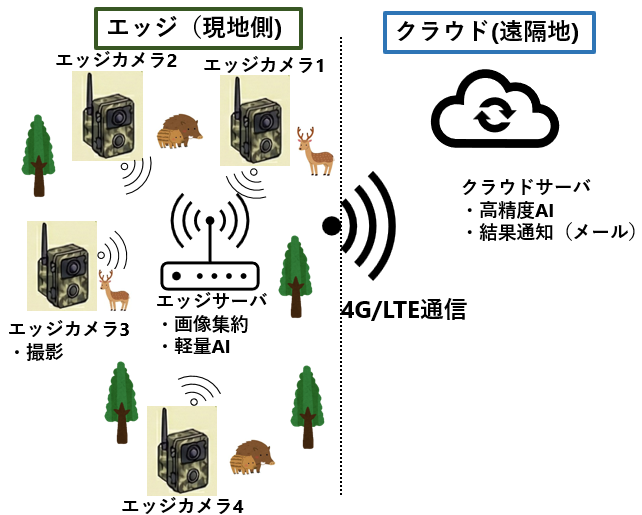
\includegraphics[width=\linewidth]{img/system_structure.png}
    \caption{提案システムの全体構成}
    \label{fig:system}
\end{figure}

\begin{figure*}[tb]
    \centering
    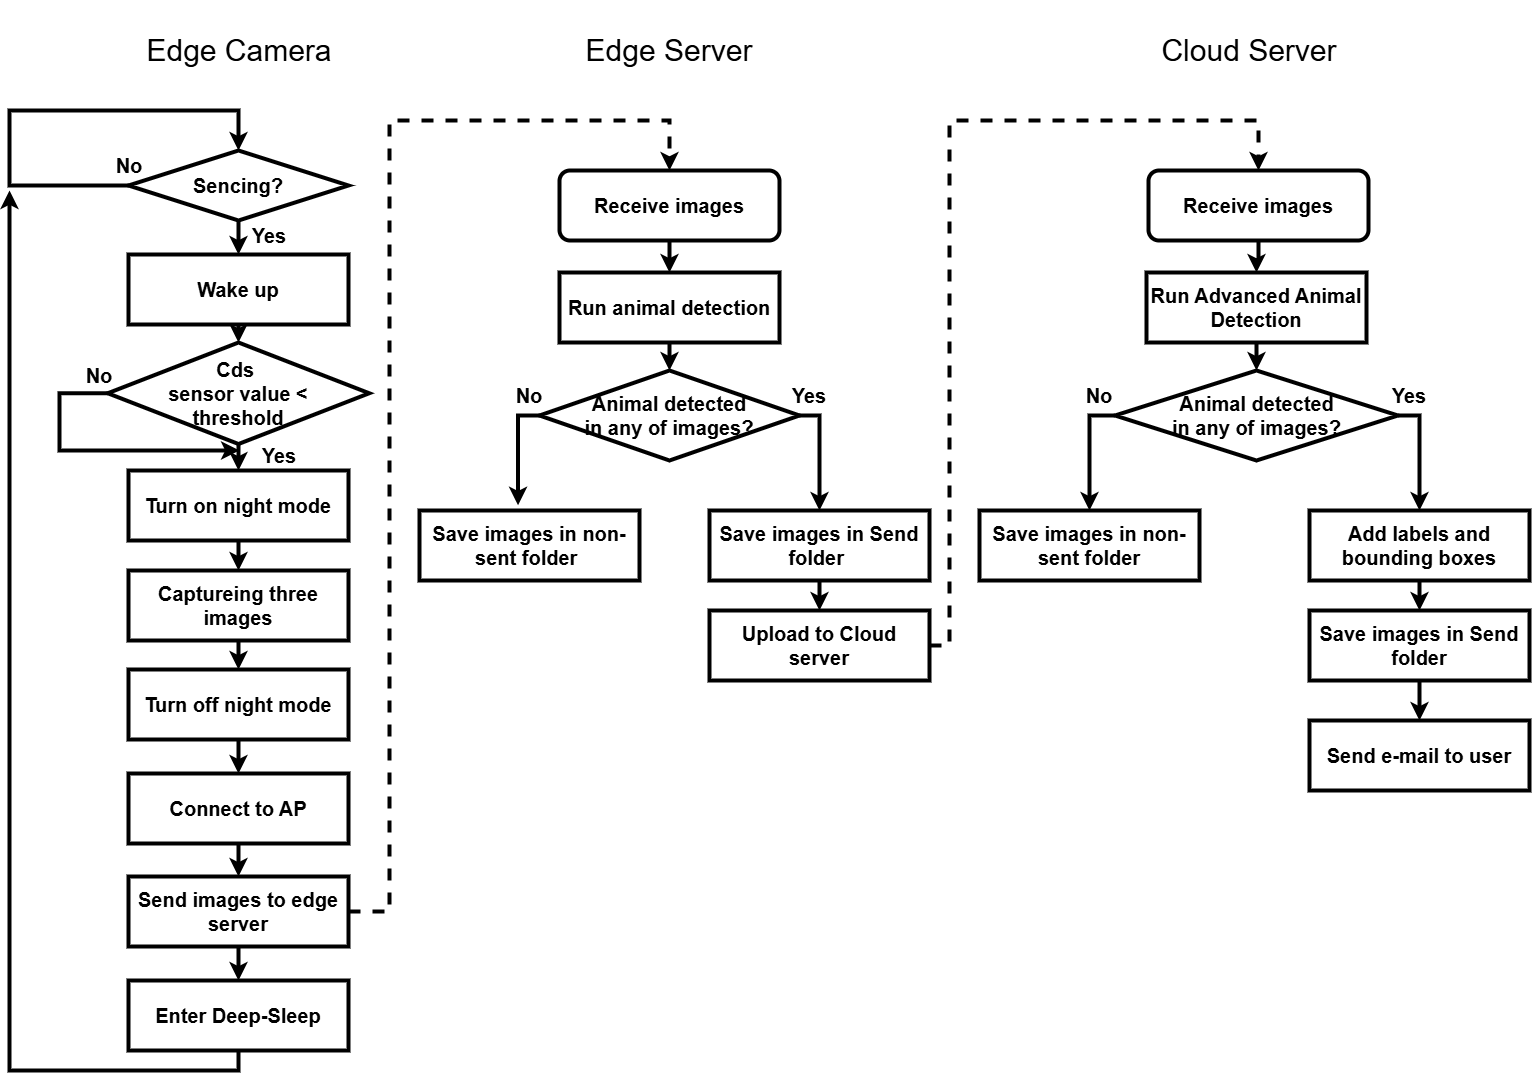
\includegraphics[width=0.85\linewidth]{img/system_flow.png}
    \caption{提案システムの処理フロー}
    \label{fig:flow}
\end{figure*}

以下に各層ごとの詳細を述べる．

\subsection{構成要素の詳細}

\subsubsection{エッジカメラ}
エッジカメラは，動物の検知と画像の取得，およびエッジサーバへのローカル通信のみを担当する．
デバイスにはSeeed Studio製のXIAO ESP32S3 Senseを採用した（図\ref{fig:camera}）．
本デバイスは安価でありながらWi-Fi通信機能とカメラ機能を備え，Deep Sleep機能により待機時の消費電力を極小化できる．
電源には単3電池8本(6V)を使用し，電源インフラのない場所への設置を容易にしている．

\textbf{処理フロー}:
常時はDeep Sleepモードで待機し，PIRセンサが熱源を検知した瞬間にウェイクアップする．
起動後，バースト撮影により連続して3枚の画像を撮影し，Wi-Fi経由でHTTP通信（POSTメソッド）を用いて直ちにエッジサーバへ送信する．
送信完了後30秒のインターバルの後，直ちにDeep Sleepモードへ移行し，バッテリー消費を抑制する．

\subsubsection{エッジサーバ}
エッジサーバは複数のエッジカメラからの画像を集約し、軽量AIによる画像選別を行い、クラウドサーバへ転送する．
シングルボードコンピュータRaspberry Pi 4Bを使用し，電源には10Wソーラーパネルと25Ahの大容量バッテリーを搭載したHyke Solar Power Pack (HC-10W25A) を採用した．
これにより，消費電力の大きいRaspberry Piの無日照下での長時間稼働を担保している．
通信モジュールとしてLTEルータ（NEC Aterm HT100LN）を接続し，クラウドとの通信を行う．

\textbf{処理フロー}:
エッジカメラからの画像受信を常時待ち受ける．
画像を受信すると，COCOデータセットで事前学習済みのYOLOv8nを用いて推論を行う．
3枚の画像のうち1枚でも動物クラスが検出された場合のみ，画像を保存用ディレクトリに移動しクラウドサーバへ転送する．
動物が検出されなかった場合（草木の揺れ等による空撮影），画像はその場で破棄され，通信帯域を消費しない．

\subsubsection{クラウドサーバ}
クラウド環境上のサーバは，受信した画像の最終的な処理とユーザへの通知を提供する．
ここでは，より計算リソースを要する高精度モデルによる再確認を行う．
解析結果に基づき，ユーザへ画像とともにメールで動物の出現を通知する．
\textbf{処理フロー}:
エッジサーバからの画像受信を常時待ち受ける．
画像を受信すると，MegaDetectorを用いて動物の検出を行う．
動物が検出された場合のみ，ユーザへ画像とともにメールで動物の出現を通知する．
動物が検出されなかった場合（草木の揺れ等による空撮影），画像はその場で破棄される．

\begin{figure}[tb]
    \centering
    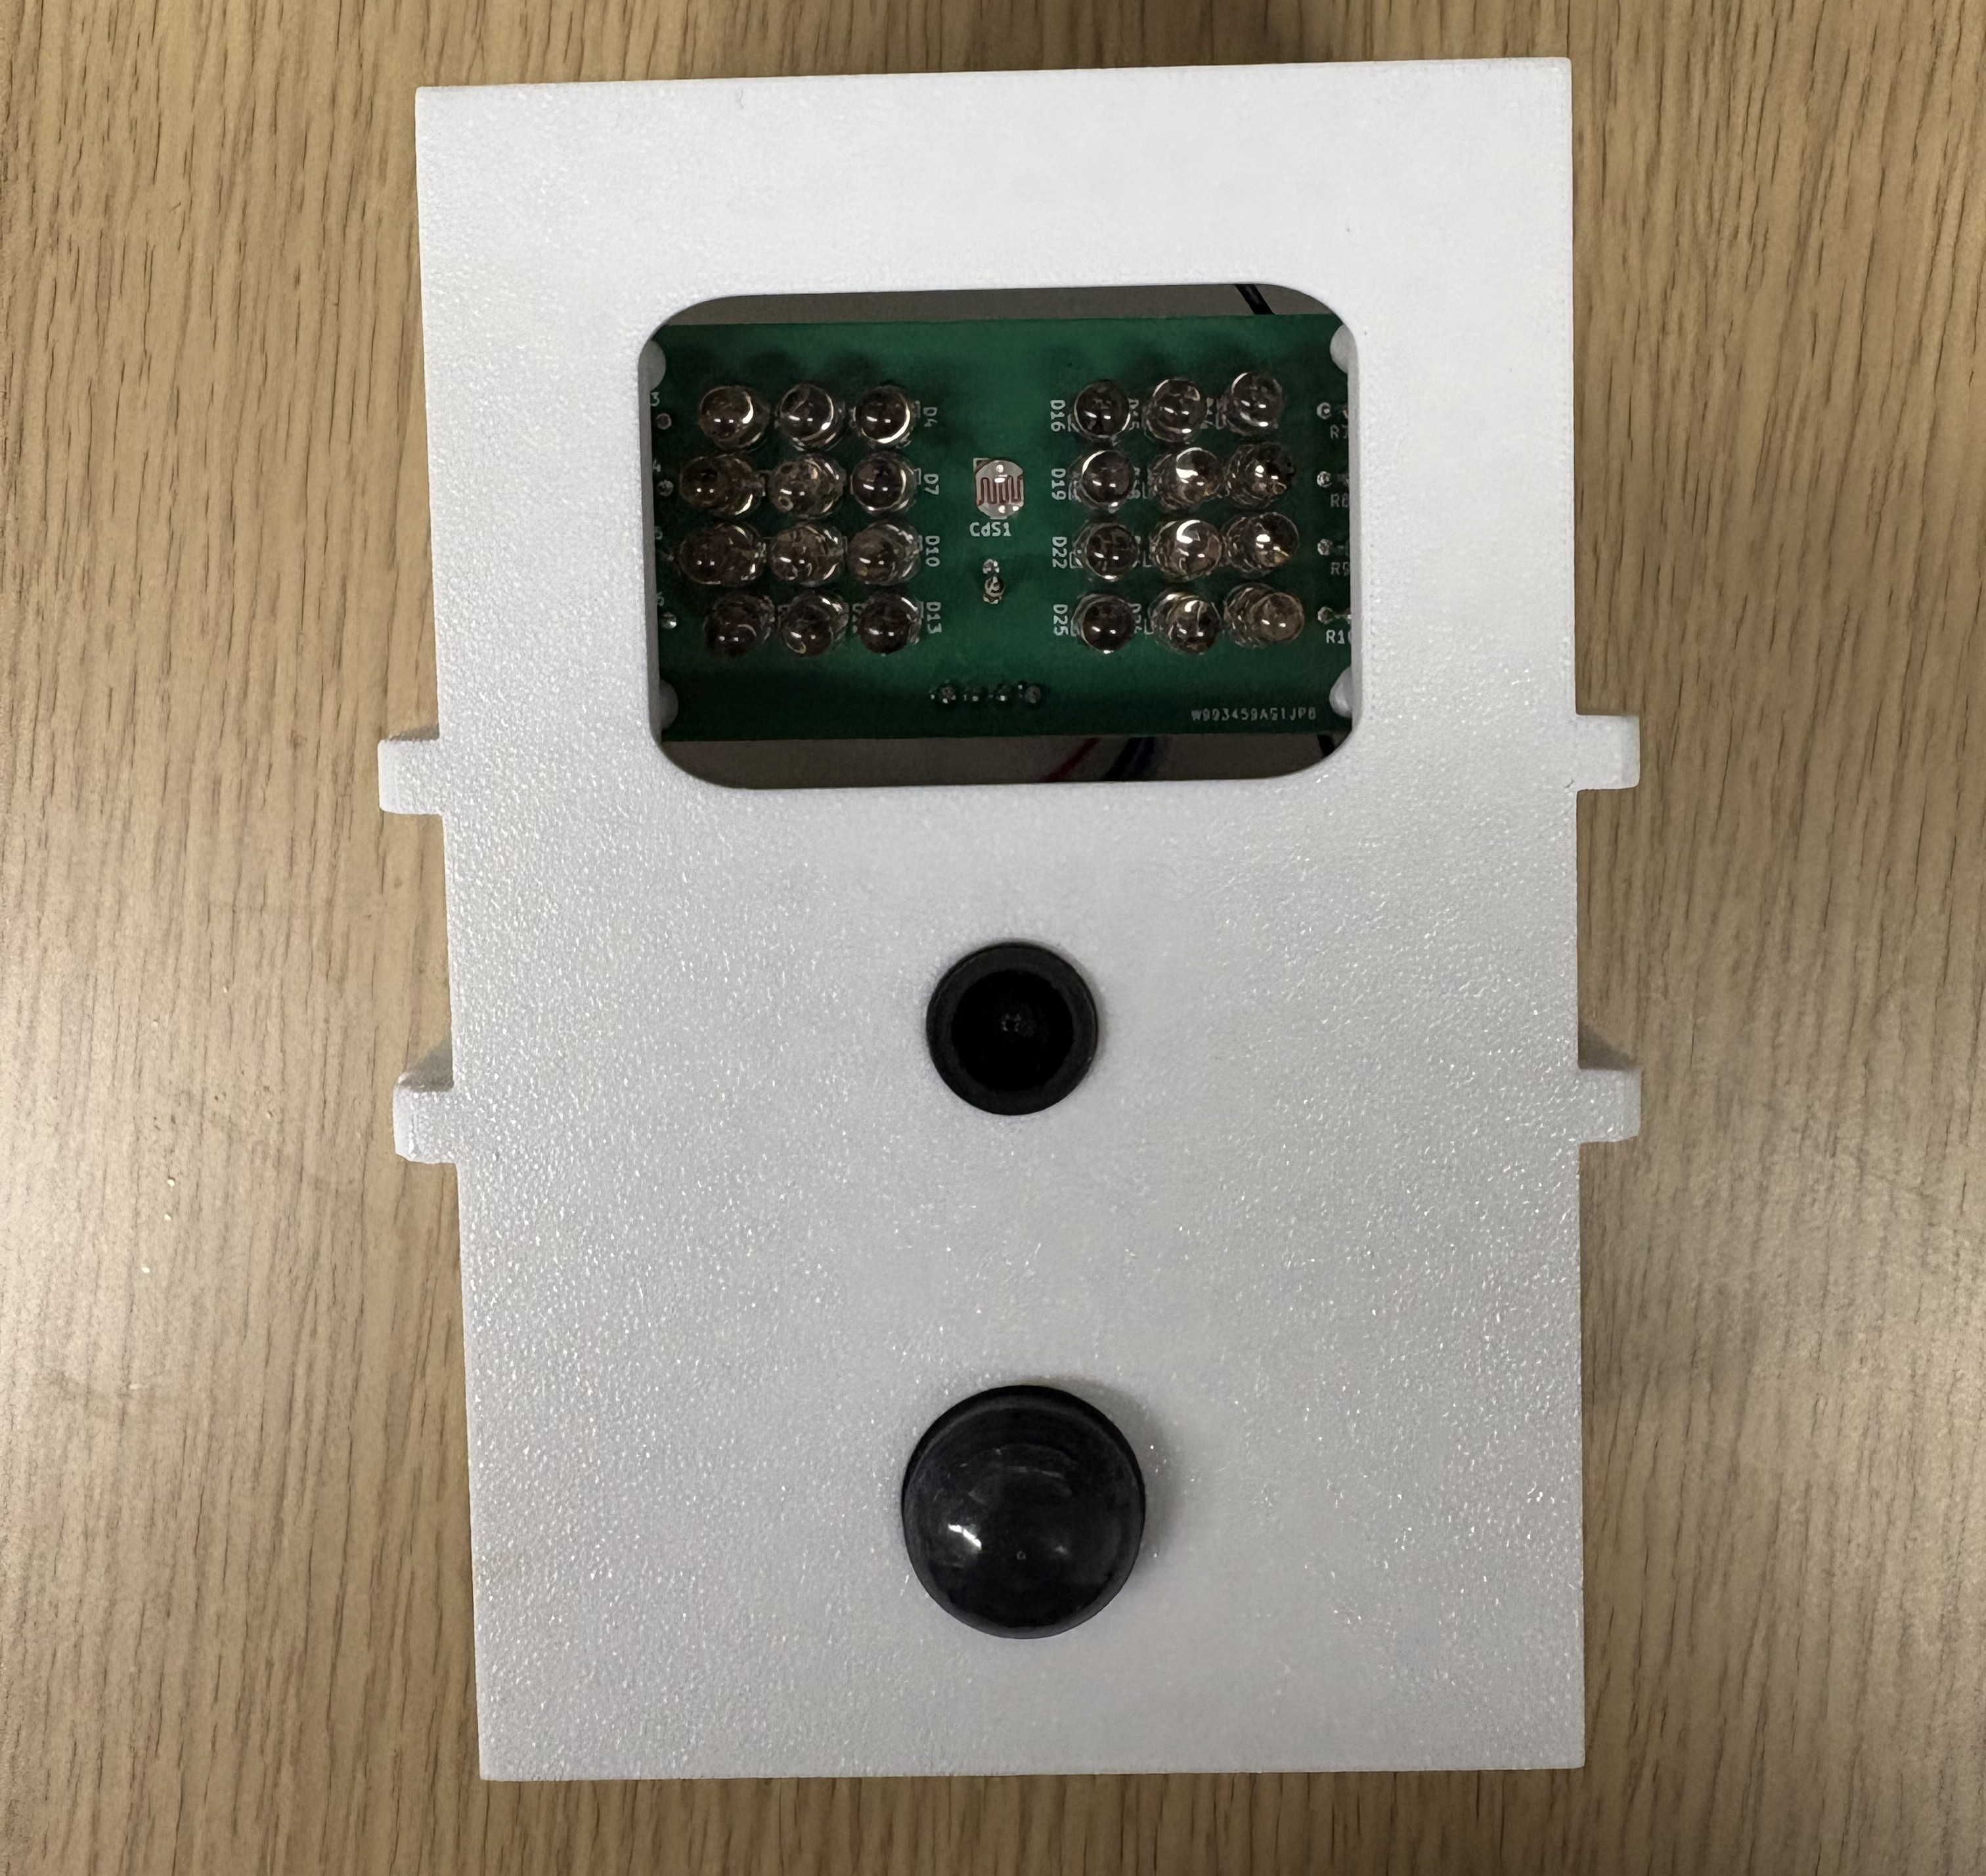
\includegraphics[width=0.6\linewidth]{img/prototype_camera.jpeg}
    \caption{エッジカメラの試作機}
    \label{fig:camera}
\end{figure}

\section{実験結果}
提案システムの実用性を検証するため，実フィールドにおける運用試験を行った．
評価項目は，1) 各ノードの基本性能（消費電力・通信性能），2) AIによるフィルタリング精度，3) システム全体の通信削減効果，および 4) エネルギー持続性である．

\subsection{実験環境とパラメータ}
実験に使用した機材構成は表\ref{tab:components}の通りである．
エッジカメラとエッジサーバは，晴天時の見通しの良い屋外環境に設置した．
エッジサーバはカメラから約5〜10mの範囲に配置し，通信テスト時は距離を変動させた．

\begin{table}[tb]
    \caption{システム構成部品}
    \label{tab:components}
    \centering
    \begin{tabular}{l|l|l}
        \hline
        構成要素     & モデル                   & 仕様           \\
        \hline \hline
        \multicolumn{3}{l}{\textbf{エッジカメラ}}                          \\
        \hline
        メインユニット     & XIAO ESP32S3 Sense      & 240MHz, 8MB PSRAM       \\
        カメラモジュール & OV5640                  & 2592$\times$1944        \\
        PIRセンサ    & Panasonic PaPIRs        & 検知範囲 $\sim$5m \\
        電源  & 単3電池 $\times$ 8 & 6V / 12V 構成         \\
        \hline \hline
        \multicolumn{3}{l}{\textbf{エッジサーバ}}                          \\
        \hline
        メインユニット     & Raspberry Pi 4B         & 4GB RAM                 \\
        電源   & Hyke Solar Power Pack   & 10W ソーラー, 25Ah バッテリー \\
        通信モジュール  & NEC Aterm HT100LN       & LTEルータ              \\
        \hline
    \end{tabular}
\end{table}

\subsection{エッジカメラの消費電力評価}
エッジカメラの各動作状態における消費電力を測定した（表\ref{tab:camera_power}）．
電源電圧5.0Vにおいて，待機時の電流は114mA，起動時の最大ピーク電流は946mAであった．
また，30秒間隔で連続動作させた場合の平均消費電流は約120mAとなった．

\begin{table}[tb]
    \caption{エッジカメラの消費電力測定結果 (5.0V)}
    \label{tab:camera_power}
    \centering
    \begin{tabular}{l|c|c}
        \hline
        動作状態        & 消費電流 (mA) & 消費電力 (W) \\
        \hline \hline
        待機時      & 114          & 0.57      \\
        起動時 (最大)   & 946          & 4.73      \\
        Wi-Fi送信時     & 250          & 1.25      \\
        30秒間隔 (平均) & 120          & 0.60      \\
        \hline
    \end{tabular}
\end{table}

\subsection{エッジサーバの消費電力評価}
エッジサーバ（Raspberry Pi 4B）についても同様に消費電力を測定した．
電源電圧5.0Vにおいて，システム起動後の安定状態（アイドル時）における消費電流は405$\sim$410mAで推移し，平均消費電力は約2.05Wであった．
なお，Raspberry Piの仕様上，安定駆動には3A以上の電源供給能力が推奨されているため，本システムではこの要件を満たす電源回路およびバッテリーを選定している．

\subsection{エッジカメラ・サーバ間の通信性能}
見通しの良い環境下において，エッジカメラとサーバ間の距離を変えながら通信安定性を評価した．
表\ref{tab:comm_perf}に実験結果を示す．
近距離（約1m）ではRSSI -30$\sim$-35dBm程度で安定して推移した．
距離を100mとした場合，RSSIは-60$\sim$-65dBm程度となり，最大距離である200m地点においては-77$\sim$-80dBmまで低下した．
しかし，いずれの条件下においてもコネクションの確立および画像の転送は問題なく完了することを確認した．

\begin{table}[tb]
    \caption{通信性能評価結果 (見通し環境)}
    \label{tab:comm_perf}
    \centering
    \begin{tabular}{c|c}
        \hline
        距離 (m) & RSSI (dBm) \\
        \hline \hline
        $\approx$ 1 & -30 $\sim$ -35 \\
        $\approx$ 100 & -60 $\sim$ -65 \\
        $\approx$ 200 & -77 $\sim$ -80 \\
        \hline
    \end{tabular}
\end{table}

\subsection{エッジサーバによるフィルタリング効果}
本研究の核となる，エッジサーバ上のYOLOv8による動物検知精度と，それによる通信量削減効果を評価する．
実験期間中に取得された画像について，目視確認および高精度モデル（MegaDetector）による判定を正解ラベル（Ground Truth）として，エッジサーバの判定精度を算出した（表\ref{tab:ai_accuracy}）．
ここで，適合率（Precision）はAIが「動物あり」と判定した画像のうち実際に動物が含まれていた割合を，再現率（Recall）は実際に動物が含まれている画像のうちAIが正しく検知できた割合を表す．

\begin{table}[tb]
    \caption{AI検知精度と環境による比較 (閾値: 0.05)}
    \label{tab:ai_accuracy}
    \centering
    \begin{tabular}{l|c|c}
        \hline
        評価指標              & 夜間 & 昼間 \\
        \hline \hline
        真陽性 (TP)  & 104          & 195        \\
        偽陽性 (FP) & 28           & 73         \\
        偽陰性 (FN) & 48           & 13         \\
        真陰性 (TN)  & 88           & 1147       \\
        適合率 (Precision)           & 78.8\%       & 72.8\%     \\
        再現率 (Recall)              & 68.4\%       & 93.8\%     \\
        見逃し率 (Miss Rate)           & 31.6\%       & 6.2\%      \\
        \hline
    \end{tabular}
\end{table}

表\ref{tab:comm_reduction}に通信削減率を示す．ここで通信削減率は，全トリガー数（PIRセンサが反応した回数）に対し，サーバが「送信不要（動物なし）」と判断して破棄した割合を示す．

\begin{equation}
    \text{通信削減率} = \left( 1 - \frac{\text{送信サイクル数}}{\text{全検知サイクル数}} \right) \times 100
\end{equation}

\begin{table}[tb]
    \caption{昼夜別の通信削減率}
    \label{tab:comm_reduction}
    \centering
    \begin{tabular}{l|c|c}
        \hline
        項目                   & 夜間 & 昼間  \\
        \hline \hline
        全検知回数 & 268   & 1428 \\
        送信回数     & 132   & 268  \\
        削減率 (\%)    & 50.7  & 81.2 \\
        \hline
    \end{tabular}
\end{table}

結果として，昼間において、再現率93.8\%、適合率72.8\%で、約81.2\%という通信削減率を達成した．
RSSI -35dBm程度の良好な通信環境において，システム全体の処理時間を計測した．
エッジ側（カメラ撮影からエッジサーバでの送信処理完了まで）の処理時間は約33秒（カメラ処理約20秒，エッジサーバ処理約13秒の合計）であった．
また，クラウド側での処理（受信からメール通知完了まで）には約11秒を要した．
結果として，動物を検知してからユーザへのメール通知が確定するまでの合計所要時間は約44秒であった．

\subsection{導入コストの比較}
本システムの有用性を検証するため，市販の鳥獣被害対策用LTEカメラ（従来機）と提案システムの導入コストを試算し比較した．
試算条件として，広範囲を監視するために5地点にカメラを設置する場合を想定する．

従来機は1台あたり約80,000円であり，5台導入する場合の初期費用は400,000円となる．また，各カメラにSIMカードが必要となるため，ランニングコストとして5回線分の通信費が発生する．

一方，提案システムにおける機材費の内訳は，エッジカメラが1台あたり約8,000円，エッジサーバ本体が約14,000円，サーバ用電源システムが約33,000円，LTEルーターが約13,000円である．
カメラ5台構成の場合，初期費用はカメラ5台分（40,000円）と，エッジサーバ・電源・ルーターの一式（60,000円）を合わせ，合計100,000円となる．
これは従来機の導入コストと比較して約75\%の削減に相当する．
さらに，通信契約はエッジサーバに接続されたルーターの1回線分のみで済むため，月々の通信費も5分の1に圧縮可能である．

\section{考察}

\subsection{通信削減効果とAI精度のトレードオフ}
実験結果（表\ref{tab:comm_reduction}）において，昼間は約81.2\%という高い通信削減率を達成した．
これは，昼間は日射による温度変化や風による植生の揺らぎ等が原因で頻繁に空撮影が発生するが，画像処理側でこれらを正しく「動物なし（True Negative）」と判定できているためである．
夜間は気温低下によりPIRセンサの誤作動自体が少ないため削減率は50\%程度となるが，それでも半数の不要データを削減できている．
全体として，本システムを導入することで，単純に全ての撮影画像を送信する場合と比較して通信量を大幅に抑制できることが定量的に示された．

なお，夜間のRecall（再現率）が68.4\%とやや低い値となっている．これはYOLOv8nという軽量モデルの限界に加え，夜間画像の画質（赤外線照射範囲やノイズ）に起因するものと考えられる．
鳥獣害対策においては見逃しを防ぐことも重要であるため、モデル学習や画像処理などで夜間画像に対しても再現率を向上させる必要がある．

\subsection{システムの実用性とコスト優位性}
通信性能の実験結果より，見通し環境下では100mの距離でも安定した通信が可能であった．
これは，一般的な農地やある程度開けた山林環境において，システムが十分なエリアカバー能力を有していることを示唆する．
また，システム全体の遅延は約44秒であり，鳥獣害対策において求められる即時性を一定水準で満たしている．
コスト面に関しては，導入コストで計算上約75\%の削減が可能であり，ランニングコストも大幅に圧縮できる．
これらにより，本システムは低コストかつ広範囲な展開が可能であり，実用性の高い監視網を構築できるといえる．

\subsection{エネルギー持続性と運用負荷}
エッジカメラの待機電力は0.57W（114mA）であり，乾電池8本による数カ月の長期間駆動は見込めない．
これは、エッジカメラのマイコンによるカメラ電源制御が不可能であるため，常にカメラが起動していることに起因する．
また，エッジサーバの消費電力は約2.05Wであるが，採用した10Wソーラーパネルと25Ahバッテリーの組み合わせにより，無日照期間が続いた場合でも理論上約60時間の連続稼働が可能である．
以上のことから，エッジサーバについては商用電源不要での持続的な運用が可能であることが確認された．
一方で，エッジカメラについては現状の消費電力では頻繁な電池交換を要するため，実用化に向けてはカメラモジュールへの給電を制御する回路の追加等のハードウェア改良が不可欠である．

\section{結論}
本論文では，広域鳥獣害対策における通信コストと運用負荷の削減を目的とし，エッジカメラ，エッジサーバ，クラウドサーバの3層構造からなる低コストな監視システムを提案した．
実フィールドにおける評価実験の結果，エッジサーバ上のYOLOv8を用いたフィルタリングにより，特に誤検知の多い昼間において約81.2\%の通信量を削減できることを示した．
また，既存のLTEトレイルカメラと比較して初期導入コストを約75\%削減できる試算となり，経済的な優位性を確認した．

一方で，エッジカメラの長期運用に関しては，Deep Sleep時の待機電力削減だけでは不十分であり，カメラモジュールへの給電制御を含むハードウェアの改良が課題として残された．
今後は，夜間の検知精度向上に向けた学習モデルの改善と，エッジノードの更なる省電力化に向けたハードウェア改良に取り組む予定である．
さらに，監視エリアの拡大に向けたLPWA (Low Power Wide Area) 通信の導入や，収集データの付加価値を高めるクラウド側での動物種判別機能の実装，およびユーザが任意に撮影リクエストやデータ閲覧を行えるWebインターフェースの構築など，システムの実用性と利便性を高める機能拡充も進めていく．

\ack
本研究を遂行するにあたり，有益な助言を頂いた信州大学の佐藤真平先生に深く感謝する．
また，実証実験のフィールド提供および多大なる協力を頂いた長野県木曽町役場の関係各位に心より感謝の意を表する．

\bibliographystyle{sieicej}
\bibliography{refs}

\appendix
%\section{}

\begin{biography}
    \profile{正員}{佐藤 光汰}{紹介文}
    %\profile{会員種別}{名前}{紹介文}% 顔写真あり
    %\profile*{会員種別}{名前}{紹介文}% 顔写真なし
\end{biography}


\end{document}
